\chapter{Αναγνώριση προσώπων}\label{ch:facerec}

Στο κεφάλαιο αυτό θα μιλήσουμε για τη διαδικασία της αναγνώρησης προσώπου. Η
διαδικασία αυτή διαφέρει από τη διαδικασία της ανίχνευσης προσώπου όσον αφορά τα
εξής:

\begin{description}
  \item[Ανίχνευση Προσώπου] \hfill \\
    Έχει ως σκοπό τον εντοπισμό προσώπων (θέση, διαστάσεις) εντός μιας εικόνας
    και πιθανότητα την εξαγωγή τους για να χρησιμοποιηθούν από τη διαδικασία της
    αναγνώρησης προσώπων

  \item[Αναγνώρηση Προσώπου] \hfill \\
    Παραλαμβάνει μια εικόνα προσώπου από την προηγούμενη διαδικασία και έχει ως
    σκοπό είτε \textbf{α)} να ταυτοποιήσει -κάνοντας μία $1x1$ σύγκριση- ότι το
    πρόσωπο αυτό ταυτίζεται με ένα συγκεκριμένο πρόσωπο που δέχθηκε ως είσοδο
    είτε \textbf{β)} να αναγνωρήσει το πρώσοπο προγματοποιώντας $1xN$ συγκρίσεις
    με ένα σύνολο από εικόνες προσώπων.

\end{description}

Η αναγνώρηση προσώπων είναι μια εύκολη διαδικασία για τον ανθρώπινο εγκέφαλο.
Έρευνες \cite{} έχουν δείξει ότι ακόμη και ένα βρέφος τριών ημερών  είναι σε
θέση να διακρίνει μεταξύ γνωστών προσώπων.Σύμφωνα με τις
εργασίες των \cite{} και \cite{} ο ανθρώπινος εγκέφαλος έχει εξειδικευμένους
νευρώνες οι οποίοι ανταποκρίνονται σε συγκεκριμένα χαρακτηριστικά μιας οπτικής
εικόνας -όπως οι γραμμές, οι ακμές, οι γωνίες και η κίνηση- και τα οποία
επεξεργάζεται καταλλήλως και δημιουργεί πρότυπα. Πάνω σε αυτό το πλαίσιο λειτουργεί
και η αναγνώριση προσώπων από υπολογιστές, στην εξαγωγή συγκεκριμένων χαρακτηριστικών
από μια εικόνα, την αναπαράστασή τους με μια αναγνωρίσιμη από υπολογιστές μορφή
και τη διενέργια κάποιου είδους ταξινόμησης μέσα από αυτά.


Η πιο συνήθης προσέγγιση είναι η αναγνώρηση προσώπων χρισιμοποιώντας κάποια
γεωμετρικά χαρακτηριστικά του προσώπου. Μια πρώτη προσέγγιση πάνω στο προαναφερθήσα
λογική περιγράφεται εδώ \cite{} όπου χαρακτηριστικά όπως τα μάτια, η μύτη, τα
αυτιά κ.α. χρησιμοποιούνται για την κατασκευή διανισμάτων σχετικά με τη θέση,
την απόσταση και τη γωνίας μεταξύ τους. Στη συνέχεια υπολογίζεται η ευκλείδια
απόσταση μεταξύ των προηγουμένως υπολογισμένων διανυσμάτων και των διανυσμάτων
μιας εικόνας με ένα γνωστό πρόσωπο. Συγκρίνοντας τις αποστάσεις με διάφορα δείγματα
το πρόσωπο που αναγνωρίζεται θεωρείται το δείγμα με την μικρότερη απόσταση. Παρόλο
που η μέθοδος αυτή δεν επιρεάζεται από τις αλλαγές στο φωτισμό, σύμφωνα με
μελέτες \cite{}, τα γεωμετρικά χαρακτηριστικά ενός προσώπου δεν παρέχουν αρκετή πληροφορία
για ακριβή αποτελέσματα.

Κατά καιρούς διάφορες μέθοδοι έχουν προταθεί. Οι πιο χαρακτηριστικές είναι:

\begin{enumerate}
    \item \emph{EigenFaces - 1991 ~\cite{}}
  \item \emph{Local Binary Patterns Histograms - 1996 ~\cite{}}
  \item \emph{FisherFaces - 1997 ~\cite{}}
  \item \emph{Scale Invariant Feature Transform (SIFT) - 1999 ~\cite{}}
  \item \emph{Speed Up Robust Features (SURF) - 2006 ~\cite{}}
\end{enumerate}

Οι μέθοδοι EigenFaces και FisherFaces, όπως και οι SIFT και SURF χρησιμοποιούν
τις ίδιες τεχνικές για την εξαγωγή των χαρακτηριστικών μιας εικόνας και τη σύγκρισή
τους με το σύνολο των εικόνων που δέχτηκαν ως είσοδο.

Παρακάτω θα δωθεί μια περιγραφή για τις τρεις πρώτες μεθόδους και να αναλυθεί
το σημείο της μεθόδου LBPH που τροποποιήθηκε στα πλαίσια αυτής της διπλωματικής.


\section{H μέθοδος EighenFaces}\label{sec:eigen}

Το πρόβλημα με την αναπαράσταση εικόνας που χρησιμοποιείται είναι ότι αναπαρίσταται
στο διανυσματικό χώρο με ένα διάνυσμα πολλών διαστάσεων. Για παράδειγμα μια ασπρόμαυρη
εικόνα δύο (2) διαστάσεων $p x q$ αναπαρίσταται με ένα διάνυσμα $m=pq$-θέσεων.
Οπότε μια εικόνα $100 x 100$ pixels παράγει ένα διάνυσμα $10,000$ θέσεων.
Στην πραγματικότητα όμως για να εξάγουμε συμπεράσματα στο εν λόγω πρόβλημα της
αναγνώρησης προσώπων δε μας είναι απαραίτητη το σύνολο της πληροφορίας που υπάρχει
σε ολόκληρη την εικόνα. Χρειάζεται να εντοπίσουμε τις υποπεριοχές της
εικόνας οι οποίες περιέχουν την πληροφορία που χρειαζόμαστε για την αναγνώρηση
του προσώπου. Η βασική ιδέα για να επιλέξουμε την πληροφορία που χρειαζόμαστε είναι
ότι ένα διάνυσμα πολλών διαστάσεων συνήθως περιγράφεται από ένα σύνολο μεταβλητών
που συσχετίζονται μεταξύ τους και επομένως χρειάζονται μόνο ορισμένες για να εξαχθεί
η πληροφορία που χρειαζόμαστε. Η παραπάνω ιδέα αναλύεται στη μέθοδο
Principal Component Analysis (PCA) η οποία προτάθηκε τόσο από τον Karl Pearson
\cite{} (1901) όσο και από τον Harold Hotelling \cite{} (1933) και περιγράφει
πως ένα σύνολο πιθανώς συσχετιζόμενων μεταβλητών περιγράφεται επαρκώς από ένα
μιρκότερο σύνολο μη-συσχετιζόμενων μεταβλητών.

\subsection{Περιγραφή του αλγορίθμου}\label{subsec:eigenalgo}

Έστω $X = \{x_1, x_2, ..., x_n\}$ ένα τυχαίο διάνυσμα όπου κάθε $x_i \in \mathbb{R}^d$

\begin{enumerate}
    \item Υπολόγισε τον μέσο $\mu$
        \begin{equation}
            \mu = \frac{1}{n}\sum_{i=1}^{n} x_i
            \tag{1}
        \end{equation}

    \item Υπολόγισε την μήτρα συνδιακύμανσης $S$
        \begin{equation}
            S = \frac{1}{n}\sum_{i=1}^{n} (x_i-\mu)(x_i-\mu)^T
            \tag{2}
        \end{equation}

    \item Υπολόγισε τις ιδιοτιμές (eighenvalues) $ \lambda_i $ και τα ιδιοδιανύσματα (eighenvectors) $ v_i $
        \begin{equation}
            Sv_i = \lambda_i v_i
            \tag{3}
        \end{equation}

    \item Ταξινόμησε τα ιδιοδιανύσματα σε φθίνουσα σειρά σύμφωνα με τις ιδιοτιμές τους. Τα $ k $ κυριότερα στοιχεία
        είναι τα ιδιοδιανύσματα που αντιστοιχούν στις $ k $ μεγαλύτερες ιδιοτιμές.
\end{enumerate}

Τα $ k $ κυριότερα στοιχεία του διανύσματος $ x $ δίνονται από τον ακόλουθο τύπο
\begin{equation}
    y = W^T(x-\mu)
    \tag{4}
    \label{eq:4}
\end{equation}όπου
$ W = (v_1, v_2, \ldots, v_k) $
\\
Η ανακατασκευή του διανύσματα χρησιμποιώντας τη μέθοδο PCA προκύπτει
\begin{equation}
    x = Wy + \mu
    \tag{5}
    \label{eq:5}
\end{equation}

Η αναγνώρηση του προσώπου με τη μέθοδο Eighenface γίνεται με τον εξής τρόπο:
\begin{enumerate}
    \item Αρχικά αναπαριστούμε με τη μέθοδο PCA όλες τις εικόνες που χρησιμοποιούμε ως δείγματα
        χρησιμοποιώντας την εξίσωση \ref{eq:4}
    \item Αναπαριστουμε με την μεθοδο PCA την προς αναγνωρηση εικονα με βαση την εξισωση \ref{eq:5}
    \item Συγκρινουμε την προηγουμενη αναπαρασταση με τις αναπαραστασεις των δειγματων και
        υπολογιζουμε τον κοντινοτερο γειτονα
\end{enumerate}

Απο πλευρας πολυπλοκοτητας, η μεθοδος που ακολουθησαμε εμπεριεχει ενα προβλημα
υπολογιστικου χωρου. Ας υποθεσουμε οτι μας δινονται ως δειγματα 400 εικονες
μεγεθους 100 x 100 pixels. Ακολουθωντας τη μεθοδο PCA, πρεπει να υπολογισουμε
τη μητρα συνδιακυμανσης $ S = XX^T $, οπου \emph{size(X)} = 10000 x 400. Καταληγουμε
με αυτον τον τροπο με εναν πινακα 10000 x 10000, οποιος καταλαμβανεις χωρο περιπου
\emph{0.8GB}.
Προκειμενου να μειωσουμε αυτο το χωρο, μπορουμε να χρησιμοποιησουμε από τη γραμμικη
άλγεβρα τη θέση ότι ένας πίνακας $M x N$ όπου $Μ > Ν$ μπορεί να έχει μόνο $N-1$
μη μηδενικές ιδιοδιοτιμές. Επόμενως χρησιμοποιώντας την ιδιοαποσύνθεση του $S$, $S=X^TX$
μεγέθους $NxN$ έχουμε:
\begin{equation}
    X^TXv_i = \mu_iv_i
    \tag{6}
    \label{eq:6}
\end{equation}

και από εκεί υπολογίζουμε τα ιδιοδιανύσματα $S = XX^T$ κάνοντας αριστερό πολλαπλασιαμό
πινάκων:
\begin{equation}
    XX^T(Xv_i) = \mu_i(Xv_i)
    \tag{7}
    \label{eq:7}
\end{equation}

Από τα παραγόμενα ορθογώνια ιδιοδιανύσματα, υπολογίζουμε τα αντίστοιχα ορθοκανονικά.

Τα EigenFaces οπτικοποιούνται ακολούθως:



\begin{figure}[htbp]
  \begin{center}
    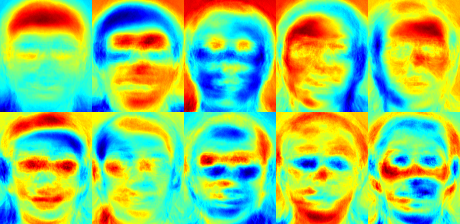
\includegraphics[width=0.8\maxwidth]{../figures/eigenfaces.png}
      \caption{EigenFaces για 10 πρόσωπα της βάσης δεδομένων AT \& T Facedatabase}\footnote{http://www.cl.cam.ac.uk/research/dtg/attarchive/facedatabase.html}
      \label{fig:eigenfaces}
   \end{center}
\end{figure}


% example
\begin{table}[htbp]
  \centering
  \begin{tabular}{ | l | l | }
    \hline
    Component & Description \\ \hline \hline
    CPU & 8 x QEMU Virtual CPU Version 1.7.0 \\
    \hline
    RAΜ & 8192 MB  \\
    \hline
    Disk & 80 GB \\
    \hline
  \end{tabular}
  \caption{Test-VM hardware specs}
  \label{tab:hw-specs}
\end{table}

\begin{table}[htbp]
  \centering
  \begin{tabular}{ | l | l | }
    \hline
    Software & Version \\ \hline \hline
    OS & Debian 7.1 Wheezy Base System \\
    \hline
    Linux Kernel & 3.2.0-4-amd64  \\
    \hline
  \end{tabular}
  \caption{Test-VM software specs}
  \label{tab:soft-specs}
\end{table}

\section{H μέθοδος FisherFaces}\label{sec:fisher}

Μία άλλη μέθοδος για τον περιορισμό της επεξεργάσιμης πληροφορία μέσα από μια
εικόνα είναι η μέθοδος FisherFaces. Η μέθοδος αυτή στηρίζεται στη γραμμική
διακριτή ανάλυση (Linear Discriminant Analysis) για τον περιορισμό των διαστάσεων
μιας εικόνας και  προτάθηκε από τον Sir R. A. Fisher \cite{}. Ο Fisher
,το 1936, ταξινόμησε με επιτυχία τα \emph{λουλούδια} ως κλάσση αντικειμένου.
Το αρνητικό της μεθόδου PCA είναι ότι είναι ευάλωτη σε εξωτερικές πηγές. Πιο
συγκεκριμένα, η μέθοδος PCA βρίσκει έναν γραμμικό συνδιασμό χαρακτηριστικών
της εικονας ο οποιος μεγιστοποιεί τη διακίμανση οφέλειμης πληροφορίας. Ο τρόπος
αυτός ενώ μας παρέχει έναν ισχυρό τρόπο αναπαράστασης της πληροφορίας, δεν λαμβάνει
υπ'όψιν την κλάσση του αντικειμένου με αποτέλεσμα διακεκριμένη πληροφορία που αφορά
τη συγκεκριμένη κλάσση αντικειμένου να χάνεται κατά τη μέθοδο. Ας υποθέσουμε ότι
εισαγεται θορυβος στην πληροφορια της εικονας απο εξωτερικο φως. Τα στοιχεια που
αναγνωριζονται απο την αναλυση PCA δεν περιεχουν απαραιτητα καποια συγκεκριμενη
πληροφορία σχετικά με το θόρυβο απο το μια εξωτερική πηγή φωτός. Αυτό καθιστά
την ταξινόμηση του προσώπου αδύνατη.
Η μεθοδος της Linear Discriminant Analysis εστιάζει στην ανεύρεση των χαρακτηριστικών
εκεινων που εντοπίζουν καλύτερα τις διαφορές μεταξύ διάφορων κλάσσεων αντικειμένων.
Η ιδεα βασιζεται στο οτι ομοιες κλασσεις ομαδοποιούνται κοντά ενώ διαφορετικές κλάσσεις
έχουν απόσταση μεταξύ τους.


\subsection{Περιγραφή του αλγορίθμου}\label{subsec:fisheralgo}

Έστω $X$ τυχαίο διάνυσμα με δείγματα από $C$ κλάσεις:
$$
X = \{X_1,X_2,\ldots,X_c\}
$$
$$
X_i = \{x_1,x_2,\ldots,x_n\}
$$

Οι διεσπαρμένοι πίνακες $S_B$ και $S_W$ υπολογίζονται ως εξής:
$$
S_B = \sum_{i=1}^{c} N_i(\mu_i-\mu)(\mu_i-\mu)^{T}
$$
$$
S_W = \sum_{i=1}^{c} \sum_{x_j \in X_i}^{} (x_j-\mu_i)(x_j-\mu_i)^{T}
$$

όπου $\mu$ είναι ο συνολικός μέσος
$$
\mu = \frac{1}{N}\sum_{i=1}^{N} x_i
$$
και $\mu_i$ είναι ο μέσος της κλάσης $i \in \{1,\ldots,c\}$
$$
\mu_i = \frac{1}{|X_i|}\sum_{x_j \in X_i} x_j
$$
Ο κλασικός αλγόριθμος του Fisher υπολογίζει την προβολή $W$ η οποία μεγιστοποιεί
το κριτήριο διαχψριστικότητας των κλάσεων ως:
%\[ \operatorname{arg\,max}_W \frac{|W^T S_B W|}{|W^T S_W W|} \]
$$
W_{opt} =
$$

Μια λύση για αυτό το πρόβλημα βελτιστοποίησης δίνεται από το γενικότερο Eigenvalue
Problem ~\cite{}
$$
S_{B}v_i = \lambda_{i}S_{w}v_i
$$
$$
S_{W}^{-1}S_{B}v_i = \lambda_{i}v_i
$$

Τα FisherFaces οπτικοποιούνται ακολούθως:


\begin{figure}[htbp]
  \begin{center}
    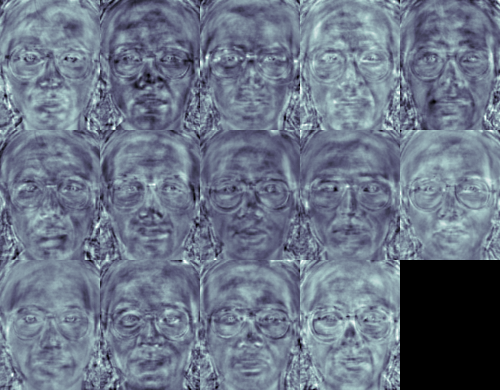
\includegraphics[width=0.5\maxwidth]{../figures/fisherfaces.png}
      \caption{FisherFaces για 16 πρόσωπα της βάσης δεδομένων Yale Facedatabase A}\flink{http://vision.ucsd.edu/content/yale-face-database}
      \label{fig:fisherfaces}
   \end{center}
\end{figure}

 The Fisherfaces method learns a class-specific transformation matrix, so the they do not capture illumination as obviously as the Eigenfaces method. The Discriminant Analysis instead finds the facial features to discriminate between the persons. It's important to mention, that the performance of the Fisherfaces heavily depends on the input data as well. Practically said: if you learn the Fisherfaces for well-illuminated pictures only and you try to recognize faces in bad-illuminated scenes, then method is likely to find the wrong components (just because those features may not be predominant on bad illuminated images). This is somewhat logical, since the :Wmethod had no chance to learn the illumination.

 The Fisherfaces allow a reconstruction of the projected image, just like the Eigenfaces did. But since we only identified the features to distinguish between subjects, you can't expect a nice reconstruction of the original image. For the Fisherfaces method we'll project the sample image onto each of the Fisherfaces instead. So you'll have a nice visualization, which feature each of the Fisherfaces describes:


\section{H μέθοδος Local Binary Patterns Histograms (LBPH)}\label{sec:lbph}

Η ιδέα πίσω από τη μέθοδο LBPH έγκειται στην εξαγωγή κάποιον τοπικών χαρακτηριστικών
από την εικόνα. Με αυτό τον τρόπο απογεύγεται η αντιμετώπιση της εικόνας ώς έναν πίνακα πολλών
διαστάσεων. Παράλληλα το γεγονός ότι βασίζεται στην ανάλυση υφής (texture analysis)
της εικόνας την καθιστά ανθεκτική σε αλλαγές στην φωτεινότητα, το μέγεθος και την
γωνία (περιστροφή) της εικόνας.

Πιο συγκεκριμένα, τα Local Binary Patterns υπολογίζουν μια τοπική δομή της εικόνας
συγκρίνοντας κάθες εικονοστεοιχείο (pixel) με τα γειτονικά του. Συγκρίνουμε την ένταση
του κεντρικού pixel με τη γειτονιά του και αντικαθιστούμε τις υπάρχουσες τιμές με
$1$ ή $0$ ανάλογα με το αν η ένταση είναι μεγαλύτερη ή μικρότερη.

Οι βασικές παράμετροι του αλγορίθμου είναι οι εξής:

\begin{description}
    \item[Radius (ακτίνα)] \hfill \\
    Έχει ως σκοπό τον εντοπισμό προσώπων (θέση, διαστάσεις) εντός μιας εικόνας
    και πιθανότητα την εξαγωγή τους για να χρησιμοποιηθούν από τη διαδικασία της
    αναγνώρησης προσώπων

    \item[Neighbors (πλήθος γειτόνων)] \hfill \\
    Παραλαμβάνει μια εικόνα προσώπου από την προηγούμενη διαδικασία και έχει ως
    σκοπό είτε \textbf{α)} να ταυτοποιήσει -κάνοντας μία $1x1$ σύγκριση- ότι το
    πρόσωπο αυτό ταυτίζεται με ένα συγκεκριμένο πρόσωπο που δέχθηκε ως είσοδο
    είτε \textbf{β)} να αναγνωρήσει το πρώσοπο προγματοποιώντας $1xN$ συγκρίσεις
    με ένα σύνολο από εικόνες προσώπων.

    \item[Grid X] \hfill \\
    \item[Grid Y] \hfill \\
\end{description}

Έτσι χρησιμοποιώντας τις προκαθορισμένες τιμές για την ακτίνα και τους γείτονες έχουμε:


\begin{figure}[htbp]
  \begin{center}
    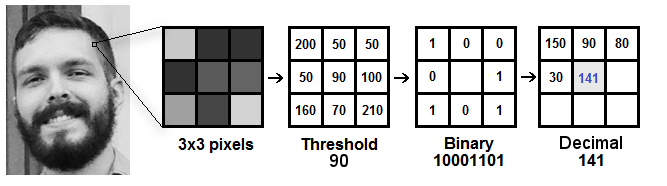
\includegraphics[width=1.0\maxwidth]{../figures/lbph1.png}
    \caption{Υπολογισμός των Locan Binary Patterns}
    \label{fig:lbph1}
  \end{center}
\end{figure}

\subsection{Default υλοποίηση}\label{subsec:lbphdef}

In order to decide which is the most appropriate candidate pool size, we
proceed with the following scenario. We sent jobs concurrently to Ganeti with
varying candidate node numbers, and we measure the rate in which jobs are
submitted to the queue, for each case.
This metric is the job enqueue throughput, and denotes the average number
of jobs that are added to the queue per second. It is a representative metric
for our purpose, because every new entry to the job queue will also be
replicated to the master candidate nodes before the operation is declared as
successful. Since we are just
interested for the enqueue rate, we decided to submit jobs that will
never be executed and will be declared as \emph{errored}. An example of those
jobs is the modification of an instance that does not exist in the cluster. The
jobs will be normally inserted to the queue and replicated to the candidate
nodes, but when they will start their execution, they will immediately fail as
\emph{errored}.

\subsection{Υλοποίση με τη χρήση του αλγορίθμου k-Nearest Neighbor}\label{subsec:lbphknn}

Jobs have been sent to Ganeti in batches of \texttt{10}, \texttt{20},
\texttt{30}, \texttt{40}, \texttt{50}, \texttt{100}, \texttt{150}, and
\texttt{200} jobs. We ran that benchmark in a \emph{5-node} cluster consisting
of \texttt{none},
\texttt{one}, \texttt{two}, and \texttt{four} master candidate nodes, and the
whole procedure has been repeated ten times in total. Since Ganeti writes every
information to filesystem and then distributes it to the candidate nodes, there
is a lot of disk and network I/O interaction. As a result, we expect a short of
deviation in our sample data values because there are external factors that may
affect the performance. The ``outliers" values that may arise should also be
included in the final results, because are part of the Ganeti behavior.
Consequently, we believe that the \emph{mean} value of our distribution is the
most appropriate metric for our case, because is a metric that represents the
\emph{central tendency} of the distribution by taking into account the whole
data information.

The benchmark outputs are summarized in two figures. Figure~\ref{fig:mc_comp},
presents the total results in a normal \emph{line-points} plot style, while
Figure~\ref{fig:const_jobs} concentrates on the heavier workload of our
benchmark that are closer to a real-world environment, in a clustered
\emph{bar-graph} plot.

\begin{figure}[htbp]
  \begin{center}
    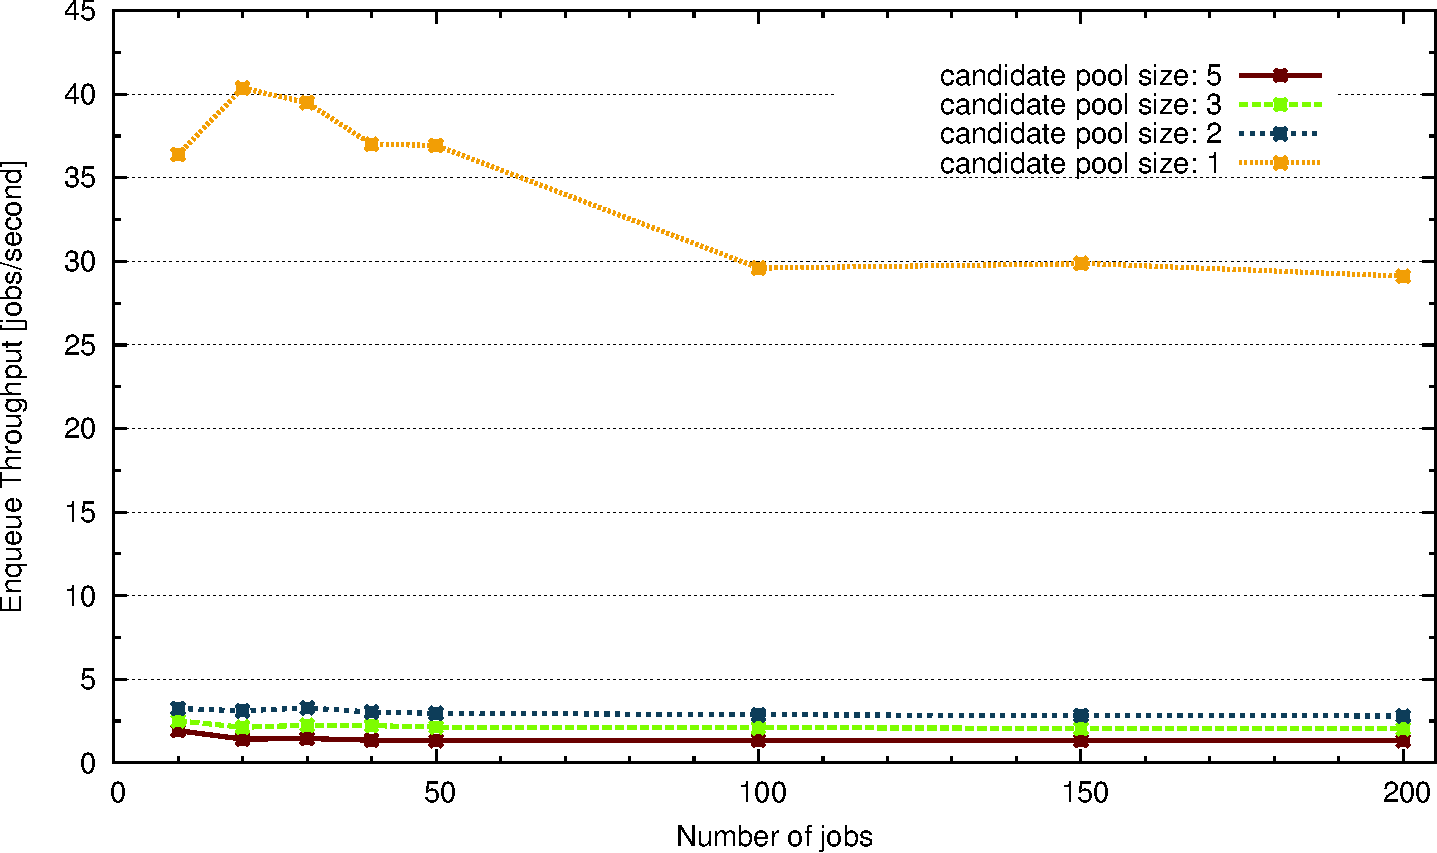
\includegraphics[width=1.0\maxwidth]{../figures/mc_comp.pdf}
    \caption{Job submission rate per number of candidates}
    \label{fig:mc_comp}
  \end{center}
\end{figure}

actors that prevent CouchDB from presenting similar behavior.


\bigskip
\newpage
\textbf{Performance Analysis}

Figure~\ref{fig:jobs_avg}, displays the average duration of the execution phases
of the \emph{InstanceCreate} jobs we submitted. For a short reminder about the
execution phases of a job, refer to Section~\ref{subsec:jobs}.

\begin{figure}[htbp]
  \begin{center}
    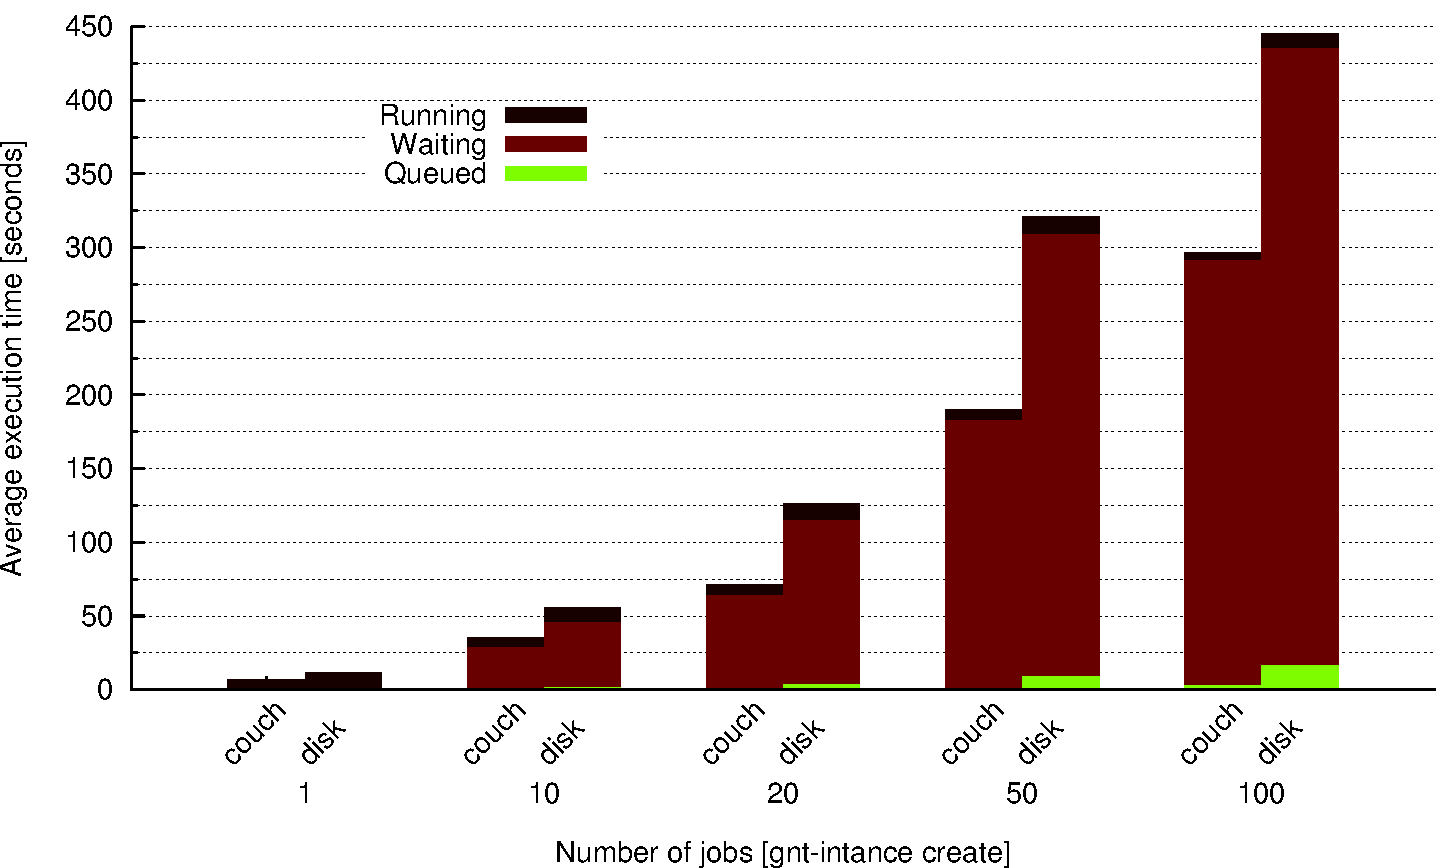
\includegraphics[width=1.0\maxwidth]{../figures/jobs_avg.pdf}
    \caption{Comparison of execution performance for the phases of a job}
    \label{fig:jobs_avg}
  \end{center}
\end{figure}

